\documentclass[a4paper,11pt,twoside,openright,pdftex]{book}
\usepackage{style/rapportPackage}
\usepackage{style/rapportlayout}

%%%%%%%%%%%%%%%%%%%%%%%%%%%%%%%%%%%%%%%%%%%%%%%%%%%%%%%%%%%%%%%%%%
\def\RapportAuthor{Elizabeth PAZ \\ Salem HARRACHE}
\def\ThesisAuthorForHyperref{Elizabeth PAZ, Salem HARRACHE}
\def\RapportTitle{Easy eLua} %project title
\def\Subtitle{eLua et approche Arduino sur STM32F4-DISCOVERY} %subtitle - if any
\def\projecttype{Projet Innovant, Avril 2012}
%%%%%%%%%%%%%%%%%%%%%%%%%%%%%%%%%%%%%%%%%%%%%%%%%%%%%%%%%%%%%%%%%%

%%%%%%%%%%%%% Change settings: (compile twice )%%%%%%%%%%%%%%%%%%%%%%
%\def\thesisversion{final}
%\def\thesislinks{no}
%\def\thesislanguage{fr}
%%%%%%%%%%%%%%%%%%%%%%%%%%%%%%%%%%%%%%%%%%

%%%%%%%%%%%%%%%%%%%%%%%%%%%% DOCUMENT %%%%%%%%%%%%%%%%%%%%%%%%%%%%
\begin{document}

\frontmatter
%\pagenumbering{alpha}
\coverpages
%%%%%%%%%%%%%%%%%%%%%%%%%%%%%%%%%%%%%%%%%%

\pagenumbering{roman}
\pagestyle{fancyplain}
\addcontentsline{toc}{chapter}{Contenu}
\tableofcontents

\addcontentsline{toc}{chapter}{Liste des figures}

\listoffigures

\addcontentsline{toc}{chapter}{Listings}

\listoftables


%%%%%%%%%%%%%%%%%%%%%%%%%%%%%%%%%%%%%%%%%%



\label{fancy:frontend} %for 'of page /x'

\clearpage{\thispagestyle{empty}\cleardoublepage}



%%%%%%%%%%%%%%%%%%%%%%%%%%%%%%%%%%%%%%%%%%%%%%%%%%%%%%%%%%%%%%%%%%

\mainmatter
\setcounter{page}{1}
\pagenumbering{arabic}
\pagestyle{fancytext}

\addcontentsline{toc}{chapter}{Introduction}
\markboth{Introduction}{}
%%%%%%%%%%%%%%%%%%%%%%%%%%%%%%%%%%%%%%%%%%%%%%%%%%%%%%%%%
\chapter*{Introduction} \label{chap:intro}

Après un quatrième semestre très chargé, l’heure est aux projets innovants. Aujourd'hui vient l'heure de l'expérience et du premier vrai test 
sur nos capacités à concevoir, à développer et à innover.

Parmi ces projets, certains, et le nôtre en particulier, s’adressent avant tout aux développeurs et aux entreprises désireuses de gagner du temps, 
et donc de l’argent. En effet, il est question ici de mettre en place une API, plus particulièrement, de porter l’API Arduino dans un autre environnement
et un autre langage.

Arduino est l’entreprise italienne qui a innové dans le monde de l’embarqué par son matériel simple, peu cher, et open source mais également par sa
 librairie qui fait passer la programmation sur embarqué pour un jeu d’enfants. Cette approche, qui consiste d’une part à offrir une structure et API 
très simple et à proposer l’ensemble en open source a aussi bien séduit les novices que les experts. Nous avons été séduits par cette approche en novices 
que nous sommes.

D'autre part, un autre projet open source dans l’embarqué prend de l’ampleur depuis quelques années: eLua. Ce projet propose un environnement Lua 
pour beaucoup de cartes microélectroniques (MicromintEagle 100, Texas instruments LM3S6965 etc.) qui permet d’écrire des programmes avec le très 
puissant langage Lua.

Notre projet repose sur ces deux projets existant pour faciliter la programmation sur les cartes STM32F4-DISCOVERY de ST-Links. Il consiste en 
le développement et portage d’une partie de l’API Arduino sur l’environnement eLua. Le but souhaité est de permettre à n’importe quel développeur
Arduino de s’y retrouver rapidement dans l’environnement eLua avec toutes les fonctions qu’il connait, déjà utilisables et exploitables.

\newpage
Ce rapport s’articule autour de trois parties. En premier lieu,  nous allons revenir sur l’approche Arduino et l’environnement eLua. 
Ensuite, nous détaillerons le déroulement du projet, la méthode de travail et le travail réalisé. Enfin on terminera par le bilan sur 
l’ensemble du projet.
%%%%%%%%%%%%%%%%%%%%%%%%%%%%%%%%%%%%%%%%%%%%%%%%%%%%%%%%%
\part{Introduction aux projets existants}
\chapter[Présentation de l’approche Arduino]{Présentation de l’approche Arduino}
\label{chap:chap2}

\section{Qu'est-ce qu'Arduino?}

\begin{figure}[h]
\begin{center}

\includegraphics[scale=0.4]{../images/Arduino/Arduinologo.png}
\caption{Logo Arduino}
\end{center}
\end{figure}

Le système Arduino \footnote{Le projet Arduino a reçu un titre honorifique à l'Ars Electronica 2006, dans la catégorie Digital Communities}
est une plateforme \textit{open-source} de programmation embarquée basée sur une carte à microcontrôleur de la famille AVR\footnote{
Cœur du processeur et famille de microcontrôleurs}, et sur un environnement
de développement intégré qui permet d'écrire, compiler et transférer un programme vers la carte. Ce logiciel utilise la technique du Processing/Wiring
\footnote{Processing est un langage de programmation et un environnement de développement}.

Avec le système Arduino on peut réaliser diverses tâches, par exemple le développement des objets interactifs indépendants : le prototypage rapide. Aussi,
la domotique, qui grâce aux différents interrupteurs/capteurs permet de contrôler plusieurs sorties matérielles : contrôle des appareils domestiques,
pilotage de robot, etc \ldots ou même charger des batteries par l'analyse et la production des signaux éléctriques.
De plus, il peut communiquer avec des logiciels tournant sur l'ordinateur tels que Macromedia Flash, Processing, MaxMSP, etc \ldots.

Le langage de programmation Arduino est une implémentation de Wiring, une plateforme de développement similaire, qui est basée sur l'environnement
multimédia de programmation Processing.

Les cartes électroniques sont accessibles à tous, elles peuvent être achetées pré-assemblées ou être fabriquées manuellement, tout en ayant la totalité des
informations nécessaires à l'assemblage.

\section{Avantages d'utilisation de Arduino}

Le système Arduino a simplifié la façon de travailler avec les microcontrôleurs, en offrant plusieurs avantages pour les enseignants, les étudiants et
les amateurs intéressés par d'autres systèmes. Ce système prend en charge des détails compliqués de la programmation des microcontrôleurs et les intègre
dans une présentation facile à utiliser. Voici, plusieurs avantages que propose Arduino :

\begin{description}
 \item[Peu coûteux:] En comparaison à d'autres plateformes les cartes Arduino sont peu coûteuses, les moins chères sont les versions qui peuvent être
assemblées à la main.
 \item[Multi-plateforme:] Le logiciel de programmation des modules Arduino est une application Java, libre et qui peut tourner dans plusieurs systèmes
d'exploitation tels que Linux, Windows et Mac.
 \item[Environnement de programmation clair et simple:] Le logiciel est facile à utiliser pour les débutants ( nous avons eu l'occasion de le tester lors de
l'initiation à l'Arduino proposé par Olivier Richard); tout en restant flexible pour des utilisations avancées.
 \item[Logiciel Open Source et extensible:] Le logiciel et le langage Arduino sont publiés sous licence Open Source et sont donc disponibles à tous, ce qui
offre la possibilité de compléter et/ou améliorer le projet. Le langage Arduino, qui utilise le langage C++, peut être étendu grâce aux librairies C++.
 \item[Matériel Open Source et extensible:] La version sur plaque d'essai de la carte Arduino peut être achetée à très bas coût et peut être montée par
n'importe quel utilisateur, elle a pour but de comprendre comment la carte fonctionne. De plus, tous les schémas de modules Arduino sont publiés. Dès lors, les
utilisateurs plus expérimentés en embarqué peuvent apporter des améliorations à leurs montages.
\end{description}


\section{Utilisation d'Arduino}

  Dans cette partie on va décrire certains points importants pour l'utilisation du logiciel, de la carte et du langage Ardduino.

\begin{figure}[h]
\begin{center}
 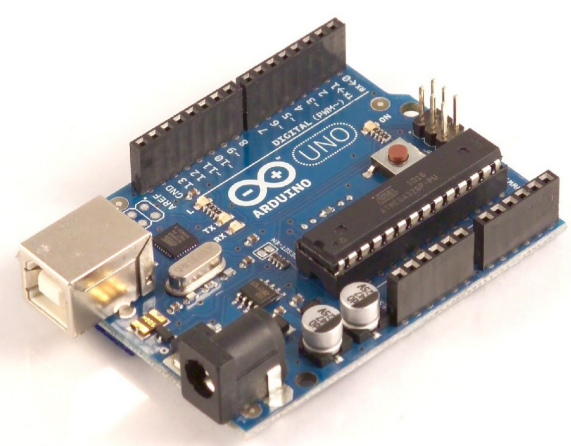
\includegraphics[scale=0.4]{../images/Arduino/arduinoUno.png}
\caption{Carte Arduino Uno}
\end{center}
\end{figure}

Un programme en langage Arduino doit obligatoirement être composé de ces deux fonctions :
\begin{itemize}
 \item la fonction d'initialisation $setup()$ qui est exécutée une seule fois au démarrage.
 \item la fonction "boucle sans fin" loop() qui est exécutée en boucle une fois que la fonction setup() a été exécutée une fois.
\end{itemize}

Puis, si besoin, d'autres fonctions peuvent être créées en suivant ce schéma :
\begin{table}[h]
\begin{lstlisting}
type nom_fonction (arguments) {
   // ici le code de la fonction
}
\end{lstlisting}
\caption{Création d'une nouvelle fonction en Arduino}
\end{table}


\begin{table}[h]
\begin{lstlisting}
/*
  Blink
  Turns on an LED on for one second, then off for one second, repeatedly.
*/
void setup() {
  // initialize the digital pin as an output.
  // Pin 13 has an LED connected on most Arduino boards:
  pinMode(13, OUTPUT);
}

void loop() {
  digitalWrite(13, HIGH);   // set the LED on
  delay(1000);              // wait for a second
  digitalWrite(13, LOW);    // set the LED off
  delay(1000);              // wait for a second
}
\end{lstlisting}
\caption{Exemple Blink pour Arduino}
\end{table}

L'utilisation du logiciel est facile et très claire, ce qui est très important à retenir c'est de bien vérifier avant d'envoyer le programme à la carte,
si on utilise le bon port et la bonne carte.

\begin{figure}[h]
\begin{center}
 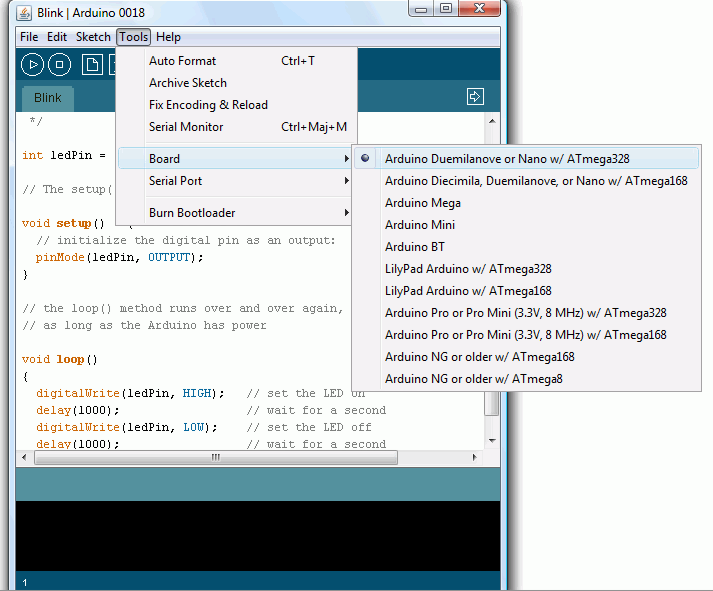
\includegraphics[scale=0.3]{../images/Arduino/logiciel.png}
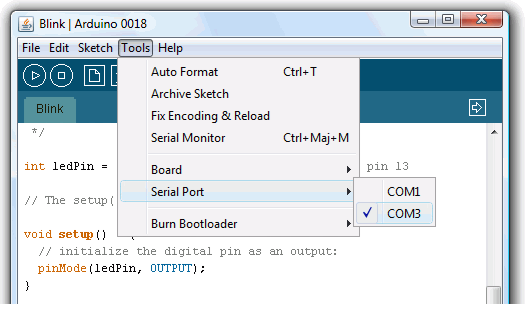
\includegraphics[scale=0.5]{../images/Arduino/logiciel1.png}
\caption{Environnement de travail: choix de la carte et du port}
\end{center}
\end{figure}

%%%%%%%%%%%%%%%%%%%%%%%%%%%%%%%%%%%%%%%%%%%%%%%%%%%%%%%%%
\chapter[Présentation d’eLua]{Présentation d’eLua}
\label{chap:chap3}

\section{À propos de Lua}

Lua est un langage de script libre, réflexif et impératif. Il a été conçu afin de pouvoir être embarqué au sein d'autres applications et les étendre.
Lua (qui signifie lune en portugais) a été développé par des membres du groupe de recherche TeCGraf, de l'université de Rio de Janeiro au Brésil.
Il est écrit en langage C ANSI strict, et de fait, il est compilable sur une grande variété de systèmes; et le plus souvent utilisé dans des systèmes
embarqués, dont sa compacité est très appréciée. De plus, il possède une compatibilité avec le langage C, c'est à dire qu'il facile d'écrire du code
C et l'exécuter dans des scripts Lua). Lua a déjà été utilisé pour le développement de jeux vidéo (beaucoup de jeux 2D de developpeurs indépendants)
ou encore comme langage de configuration du jeu World of Warcraft de Blizzard Entertainment.

\begin{figure}[h]
\begin{center}

\includegraphics[scale=1]{../images/eLua/Lua.JPG}
\caption{Logo Lua}
\end{center}
\end{figure}


\section{Qu'est-ce qu'eLua?}

  eLua adopte le langage de programmation Lua et propose une implémentation complète de celui ci pour les systemes embarqués. Il ajoute au langage de base,
une API spécifique à ces systemes pour rendre le développement de logiciels embarqués plus simples.

\subsection{Architecture de eLua}

\begin{figure}[h]
\begin{center}
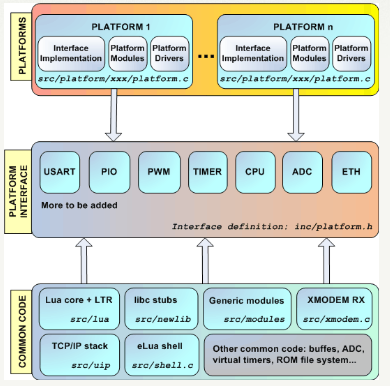
\includegraphics[scale=0.6]{../images/eLua/schema.png}
\caption{Structure logique de eLua}
\label{elua}
\end{center}
\end{figure}

  Dans la documentation d'eLua on utilise la notion de ``plateforme'' pour designer un groupe de CPU qui partagent la même structure du noyau; pourtant
ils peuvent différer dans le nombre de péripheriques integrés, la mémoire interne, et toute autres attributs. Un port eLua implemente un ou plusieurs
CPU d'une même plateforme.
Dans la figure~\ref{elua}, on observe que eLua essaie d'être aussi portable que possible dans différents plateformes, pour cela plusieurs règles ont été mises en
place, entre autre:

\begin{itemize}
 \item Le code qui est indépendant du type de plateforme doit être écrit en ANSI C dans toutes les parties ou cela est possible, afin qu'il soit
portable parmi plusieurs architectures et compilateurs, comme Lua.

 \item Le code qui ne peut pas être générique (par exemple le péripheriques et le code spécifique au CPU) doit être aussi portable que possible en
utilisant une interface en commun qui doit être implementée par toutes les plateformes dans les quelles eLua peut être executée.

 \item Toutes les plateformes et leur péripheriques ne sont pas crées de la même façon et possèdent donc des fonctionnalités très variés. Pour accèder
à une fonctionnalité spécifique à une plateforme on peut utiliser un module. Ces modules ont été crées afin de complèter l'écart entre l'interface de
la plateforme et toutes les caractéristiques proposés par la plateforme.

\end{itemize}

\subsection{Code en commun}

La liste suivante montre quelques éléments qui sont classifiés comme du code en commun:

\begin{itemize}
 \item Le code Lua
 \item Tous les composants eLua (par exemple le ROM file system, le shell eLua, et autres)
 \item Tous les modules génériques, qui sont des modules exportés de Lua
 \item Le code générique des péripheriques
\end{itemize}

C'est important de remarquer que les parties génériques doivent être la grande partie du code. Par exemple, lorsqu'on veut ajouter un nouveau fichier au système
celui-ci doit être un code générique, sinon le code aura des dependances par rapport à où il reside. On peut corriger cela en utilisant des fonctions
définies dans l'interface de la plateforme, mais si cela n'est pas possible il faudra séparer les fonctions spécifiques dans une interface separé qui va
devoir être implementée par toutes les plateformes qui veulent utiliser ce nouveau fichier. Ceci donne un maximum de portabilité au code.

L'utilisateur ne doit jamais oublier le but principal de eLua: la flexibilité. Il doit donc être dans la capacité de savoir quelles composants font partie
de son binaire eLua.

\section{Avantages de eLua}

\begin{description}

 \item[Contrôle total de la plateforme:] il n'existe pas un systèmee d'exploitation entre les programmes et le microcontrôleur.

 \item[Portabilité du code:] Comme Lua, le programme peut être executé dans un grand nombre de plateformes et d'architectures.

 \item[Facilité de transformation:] Le code et la conception des applications pour eLua peuvent être indépendant du matériel.

 \item[Développement autonome:] Lua est complètement fonctionnel avec la possibilité d'avoir un shell dans le microcontrôleur, il n'y a pas besoin
de rien installer côté ordinateur a part la connexion du port. Les programmes sont utilisable directement sur la carte microcontrôleur.

 \item[Flexibilité:] L'utilisation de ce lua comme langage de script de haut niveau dans un projet rend celui-ci très adaptable, facilement
reprogrammable et reconfigurable. Les systèmes sont très efficients pour une future évolution.

 \item[Apprendre l'embarqué: ] L'experimentation est très simple et interactive.

 \item[Open Source:] elua est libre, gratuit, et open source, comme Lua, il possède une licence MIT.
\end{description}






%%%%%%%%%%%%%%%%%%%%%%%%%%%%%%%%%%%%%%%%%%%%%%%%%%%%%%%%%
\part{Travail réalisé}
\newpage
Avant de nous attarder sur le travail réalisé, nous allons tout d’abord aborder les méthodes de travail et notre organisation tout au long pour mener à bien ce projet. Puis nous détaillerons la structure du projet et les différentes composantes de celui-ci.  Nous détaillerons enfin les fonctions portées, les fonctions qu’ils restent à écrire et les concepts nouveaux, propres à Easy-eLua. Nous terminerons  par des exemples de programme développés avec Easy-eLua

\chapter[Organisation du travail]{Organisation du travail}
\label{chap:chap5}

Sur ce projet, il y a eu deux phases distinctes. La première phase concernait la recherche d’information et l’évaluation de la 
faisabilité du projet. Cette phase était assez longue et peu productive en code.  C’est également dans cette phase où l’on a commencé 
l’initiation à la programmation de l’embarqué et l’évaluation des différentes librairies disponibles pour linux (stlink, libopenstm32...).
 Nous nous concertions avec le tuteur pour jauger la voie à emprunter, car il faut bien le dire, beaucoup de sprint n’aboutissait 
pas forcément à un résultat espéré.

Avec le recul, on peut voir cette phase comme une longue formation aux différents outils et à la programmation de l’embarqué.
Elle est d’autant plus importante, qu’elle a permis à cette d’avoir une deuxième phase très rapide. 

Pour la deuxième phase, nous avons utilisé une méthode de travail qui s'inspire des méthodes agiles. Cette méthode s'appuie sur des 
valeurs fondamentales :

\begin{itemize}
 \item Les interactions entre individus priment sur les processus et outils, ceci permet de développer davantage le travail en groupe, et favorise la communication en face à face. 
 \item Le fonctionnement prime sur le reste: il est vital que l'application fonctionne. Le reste, et notamment la documentation technique, 
est une aide précieuse mais non un but en soi.
 \item Accepter le changement plutôt que de suivre un plan. En effet, il faut considérer le changement comme une opportunité car effectuer un changement au plus tôt  permet de réduire le coût. 
\end{itemize}
 
Ceci se traduit concrètement, par des objectifs courts, les ``sprints'' qu'on se fixe en fin de semaine pour la semaine à venir. Chaque fin de journée, on se regroupe durant 15-20 minutes pour une réunion hebdomadaire. À tour de rôle, chaque développeur prend la parole pour faire part de l’avancement de son projet et peut aborder les problèmes rencontrés.
Cela nous permet de connaître l’état d’avancement de l’autre développeur et de proposer des suggestions et un nouveau point de vue. Ça permet
aussi de voir si quelqu'un est bloqué, mais généralement si c'est le cas, l'aide survient plus tôt.

À la fin de chaque sprint, on effectue une réunion où l'on dresse le  bilan de ce qui a été réalisé puis l'on fixe les objectifs du sprint suivant. 
Il n’y a pas réellement de scrum master, vu qu’on est deux et avec le même niveau de connaissances. On décide tous les deux des sprints de chacun.
%%%%%%%%%%%%%%%%%%%%%%%%%%%%%%%%%%%%%%%%%%%%%%%%%%%%%%%%%
\chapter[Arborescence du projet]{Arborescence du projet}
\label{chap:chap7}

L'arborescence du projet est la suivante :

\begin{figure}[h]
\begin{center}
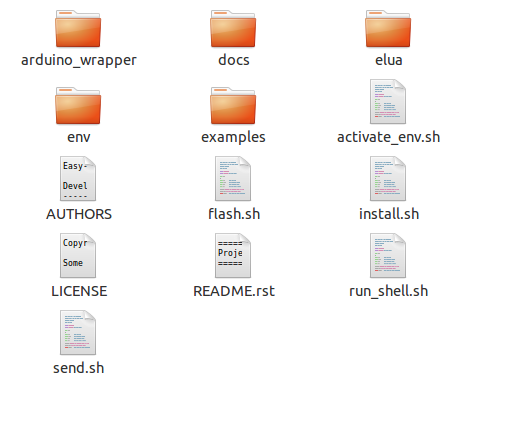
\includegraphics[scale=0.6]{../images/arborescence.png}
\caption{Arborescence du projet}
\end{center}
\end{figure}

\begin{description}
 \item[arduino\_wrapper: ] les sources de nos portages.
 \item[docs: ] contient l’ensemble des documents utiles des projets.
 \item[elua: ] contient les sources eLua.
 \item[env: ] le dossier contient les outils indispensables pour la compilation (sourcerytoolchain g++) et le flash de la carte.
 \item[examples: ] contient les exemples documentés prêts à l’emploi.
\end{description}

L’une des fonctionnalités intéressantes du projet, est l’installation automatique de l’environnement de développement.
En effet, le script ``install.sh'' permet d’automatiser cette tâche rendant plus simple le premier contact avec Easy-eLua.

Nous avons également développé d’autres scripts pour automatiser d’autres tâches, comme le flash de la carte avec un programme
Easy-eLua ou encore l’envoi de celui-ci sur une carte possédant déjà un environnement eLua.

%%%%%%%%%%%%%%%%%%%%%%%%%%%%%%%%%%%%%%%%%%%%%%%%%%%%%%%%%
\chapter[Fonctions portées]{Fonctions portées}
\label{chap:chap6}


L'environnement eLua est très riche.
La plupart des portages qu’on a réalisés sont assez courts et dépassent rarement les 10 lignes. Voici les principales fonctions portées.

\section{Entrées/Sorties numériques}

Ce sont les fonctions de base d’entrée sortie qui vont permettre d’interagir avec l’extérieur.  Trois fonctions ont été réalisées: 

\begin{description}
 \item[pinMode(): ] Cette fonction spécifie le mode (INPUT ou OUTPUT) d’une broche. 
Cette fonction existe déjà dans eLua, mais elle porte un autre nom, le portage est donc très court:

\begin{table}[h]
\begin{lstlisting}
function pinMode(pin, mode)
    if mode == OUTPUT or mode == INPUT then
        pio.pin.setdir(mode, pin)
    end
end
\end{lstlisting}
\caption{Fonction $pinMode$}
\end{table}

\item[digitalWrite(): ] Envoie la valeur HIGH ou LOW (respectivement 1 ou 0) sur une broche. De même que $pinMode()$ 
le portage ne pose pas de problème puisque cette fonction (comme on peut s’en douter) est disponible dans l’environnement eLua.
\newpage
\begin{table}[h]
\begin{lstlisting}
Function digitalWrite(pin, value)
    if value == HIGH or value == LOW then
        pio.pin.setval( value, pin )
    end
end
\end{lstlisting}
\caption{Fonction $digitalWrite$}
\end{table}

\item[digitalRead(): ] DigitalRead permet de lire la valeur de la broche. Cette valeur est soit de 0 soit de 1.
\begin{table}[h]
\begin{lstlisting}
functiondigitalRead(pin)
    return pio.pin.getval( pin )
end
\end{lstlisting}
\caption{Fonction $digitalRead$}
\end{table}


\end{description}

\section{Communication série}

Pour l'entrée/sortie série, nous avons implémenté la classe Serial proposée par Arduino.

\begin{table}[h]
\begin{lstlisting}
-- Serial communication object
SerialPort=Class:new()

function SerialPort:__new(uartid, baud,databits, parity,stopbits)
    -- Initialize SerialPort
    self.uartid = uartid
    self.baud = baud or 115200
    self.databits = databits or 8
    self.parity= parity or uart.PAR_NONE
    self.stopbits=stopbits or uart.STOP_1
end
\end{lstlisting}
\caption{Entrée/Sortie}
\end{table}

La carte STM32F4-DISCOVERY dispose de 6 modules UART (Universal Asynchronous Receiver Transmitter) dont deux synchrones (USART).
 Dans la librairie Arduino, ces modules peuvent être utilisés par des objets nommés \textbf{Serialx} où x est l’identifiant de l’UART. 
Nous disposons donc dans Easy-eLua de 6 objets Serial accessibles directement depuis le programme, puisqu’ils sont initialisés 
directement dans le fichier \textit{arduino\_wrapper.lua}.

\begin{table}[h]
\begin{lstlisting}
-- Define Serials object
Serial0 =SerialPort:new(0)
Serial1 =SerialPort:new(1)
Serial2 =SerialPort:new(2)
Serial3 =SerialPort:new(3)
Serial4 =SerialPort:new(4)
Serial5 =SerialPort:new(5)
\end{lstlisting}
\caption{Objets Serial}
\end{table}

\newpage
La classe dispose bien évidemment d’une méthode $begin()$
qui initialise la connexion série. Dans ce cas les broches ne peuvent plus être utilisées avec $digitalWrite()$ et $digitalRead()$.

\begin{table}[h]
\begin{lstlisting}
function SerialPort:begin(baud)
    -- Setup the serial port
    -- Returns: The actual baud rate set on the serial port.
    -- Depending on the hardware, this might have a different value than
    -- thebaud parameter
    self.baud = baud or self.baud
    return uart.setup(self.uartid,self.baud,self.databits,self.parity,
                                                          self.stopbits)
end
\end{lstlisting}
\caption{Fonction $begin$}
\end{table}

La fonction la plus intéressante (nous ne détaillerons pas les autres ici) c’est bien évidemment la fonction $print()$ 
qui permet d’envoyer des données avec différents formatages possibles:
\newpage
\begin{table}[h!]
\begin{lstlisting}
functionSerialPort:print(value,format)
    -- Prints data to the serial port as human-readable ASCII text.
    -- This method can take many forms. Numbers are printed using an ASCII
    -- character for each digit. Floats are similarly printed as ASCII digits,
    -- defaulting to two decimal places. Bytes are sent as a single character.
    -- Characters and strings are sent as is. For example:
    -- SerialPort.print(78) gives "78"
    -- SerialPort.print(1.23456) gives "1.23"
    -- SerialPort.print('N') gives "N"
    -- SerialPort.print("Hello world.") gives "Hello world."

    -- An optional second parameter specifies the base (format) to use;
    -- permitted values are BIN (binary, or base 2), OCT (octal, or base 8),
    -- DEC (decimal, or base 10), HEX (hexadecimal, or base 16). 
    -- For floating point numbers, this parameter specifies
    -- the number of decimal places  to use. For example:
    -- SerialPort.print(78, BIN) gives "1001110"
    -- SerialPort.print(78, OCT) gives "116"
    -- SerialPort.print(78, DEC) gives "78"
    -- SerialPort.print(78, HEX) gives "4E"
    -- SerialPort.println(1.23456, 0) gives "1"
    -- SerialPort.println(1.23456, 2) gives "1.23"
    -- SerialPort.println(1.23456, 4) gives "1.2346"

    if value == nil then
        return
    end

    if type(value) == "string" then
        uart.write(self.uartid, value)
    end

    if type(value) == "number" then
        if format ~= nil then
            if format == BIN then
                value = numberstring(value,2)
            elseif format == OCT then
                value = numberstring(value,8)
            elseif format == DEC then
                value = numberstring(value,10)
            elseif format == HEX then
                value=string.upper(numberstring(value,16))
            end
        elseif type(format) == "number" and format>=0 then
            value=string.format("%."..format.."f", value)
        else
            -- if value is float
            if value ~= floor(value)then
                value = string.format("%.2f", value)
            else
                value = string.format("%d", value)
            end
        end
        uart.write(self.uartid, value)
    end
end
\end{lstlisting}
\caption{Fonction $print$}
\end{table}
\newpage
Nous sommes restés le plus fidèle possible à la fonction initiale de Arduino.




%%%%%%%%%%%%%%%%%%%%%%%%%%%%%%%%%%%%%%%%%%%%%%%%%%%%%%%%%
\chapter[Nouveaux concepts]{Nouveaux concepts}

La structure générale d'un programme Arduino repose sur les méthodes setup() et loop().
Le méthode loop() qui constitue le cœur du programme sera appelée indéfiniment, tandis que la méthode setup() elle, 
sert seulement à initialiser les variables et le contexte d'exécution au début du programme.

Partant de ce constat, on a décidé de donner une orientation objet à nos programmes lua. En effet 
ce choix peut être contestable, mais il nous est paru important pour mettre en place une API efficace.

Lua n'est pas pourvu de type ``class'', mais il permet de programmer le comportement de ses propres objets/types. 
Autrement dit, il est certes très léger, mais c'est un langage tout désigné pour la méta-programmation. 
Le mécanisme de classe, et d’héritage est défini par les lignes suivantes:

\begin{table}[h]
\begin{lstlisting}
function Class:new(super)
    local class,metatable, properties = {},{},{}
    class.metatable=metatable
    class.properties=properties

    function metatable:__index(key)
        local prop = properties[key]
        if prop then
            return prop.get(self)
        elseif class[key] ~=nil then
            return class[key]
        elseif super then
            return super.metatable.__index(self, key)
        else
            return nil
        end
    end

    function metatable:__newindex(key, value)
        local prop = properties[key]
        if prop then
            return prop.set(self, value)
        elseif super then
            return super.metatable.__newindex(self, key, value)
        else
            rawset(self, key, value)
        end
    end

    functionclass:new(...)
        local obj=setmetatable({},self.metatable)
        if obj.__new then
            obj:__new(...)
	end
        return obj
    end
    return class
end
\end{lstlisting}
\caption{Définition du type $Class$}
\end{table} 

\newpage

Grâce à ce nouveau type, nous avons défini la classe série (vu plus haut) mais également la classe centrale: App

\begin{table}[h]
\begin{lstlisting}
-- App
App = Class:new()

function App:__new(name)
    -- Initialize App
    self.name = name
end

function App:setup()
    return
end

function App:loop()
    return
end

function App:run()
    self:println("Run : ".. self.name)
    self:setup()
    while self:condition()do
        self:loop()
    end
    collectgarbage()
end
\end{lstlisting}
\caption{Classe centrale $App$}
\end{table}

Un programme utilisant Easy-eLua n’aura qu'à redéfinir le comportement de setup() et de loop() (voir les exemples dans le chapitre ~\ref{exemples}). 
Ce qu'il faut faire en plus par rapport au modèle Arduino, est l’instanciation d’un nouvel objet $App$, puis on l'appelle à la méthode run(). 
Le lancement est donc explicite. L’idée sous-jacente est la possibilité d’avoir plusieurs applications dans un même programme.
Et le choix de laquelle lancer pourra se faire sur certaines conditions. 

\section{Fonctions relatives au temps}

Deux fonctionnalités intéressantes pour un programme ont été mises au point. 
La première est la durée d’exécution du programme. Depuis combien de temps il tourne. Ça permet généralement de différer dans le temps 
certaines tâches. La seconde est la possibilité d'attendre passivement (delay()), ce qui est vital si on ne veut pas surcharger le CPU 
(attente active avec un while).

Ces fonctionnalités sont plus au moins disponibles dans eLua.
\newpage
\begin{table}[h]
\begin{lstlisting}
function delay(period)
    -- period in milliseconds
    tmr.delay(0,period*1000)
end

function delayMicroseconds(period)
    -- period in us
    tmr.delay(0, period)
end
\end{lstlisting}
\caption{Fonction $delay$}
\end{table}

L'implémentation utilise le module timer de eLua. Lors du lancement de l'application, 
on mémorise le compteur d’un timer, pour que l'on puisse retrouver, par différence, la durée d'exécution:

\begin{table}[h]
\begin{lstlisting}
function App:run()
    self:println("Run : ".. self.name)
    self.start_counter=tmr.start(self.timerid)
    [...]
end
function App:micros()
    -- Number of microseconds since the program started
    time_now=tmr.read(self.timerid)
    return tmr.gettimediff(self.timerid,self.start_counter,time_now)
end
\end{lstlisting}
\caption{Utilisation du module timer}
\end{table}

\section{Le Shell}

Le Shell est un des avantages indéniables de l'environnement lua. On peut l'utiliser pour exécuter un interprète 
lua qui tourne directement sur la carte. On peut ainsi écrire des programmes dynamiquement, et par extension utiliser Easy-eLua par ce moyen.

Voici un exemple ``HelloWorld'' utilisant Easy-eLua: 

\begin{table}[h]
\begin{lstlisting}
eLua#lua
Press CTRL+Z to exitLua
Lua5.1.4  Copyright(C)1994-2011 Lua.org, PUC-Rio
>require("arduino_wraper")
>app=App:new("Hello World!")
>app:run()
Run: Hello World
\end{lstlisting}
\caption{Exemple ``Helllo World''}
\end{table}





%%%%%%%%%%%%%%%%%%%%%%%%%%%%%%%%%%%%%%%%%%%%%%%%%%%%%%%%%
\chapter[Exemples]{Exemples} 
\label{exemples}
\section{Blink}

\subsection{Version Arduino}

\begin{table}[h]
\begin{lstlisting}
/*
  Blink
Turns on an LED on for one second, then off for one second, repeatedly.

  This example code is in the public domain.
 */

// Pin 13 has an LED connected on most Arduino boards.
// give it a name:
int led =13;

// the setup routine runs once when you press reset:
void setup(){
    // initialize the digital pin as an output.
    pinMode(led, OUTPUT);
}

// the loop routine runs over and over again forever:
void loop(){
    digitalWrite(led, HIGH);// turn the LED on (HIGH is the voltage level)
    delay(1000);// wait for a second
    digitalWrite(led, LOW);// turn the LED off by making the voltage LOW
    delay(1000);// wait for a second
}
\end{lstlisting}
\caption{Blink: version Arduino}
\end{table}

\subsection{Version Easy-eLua}

\begin{table}[h]
\begin{lstlisting}
--  Blink
--  Turns on an LED on for one second, then off for one second, repeatedly.
require("arduino_wraper")

functionApp:setup()
    self.ledpin= ORANGE_LED -- Pin PD_13 has a LED connected
    pinMode(self.ledpin, OUTPUT)-- Initialize the digital pin as an output.
end

functionApp:loop()
    digitalWrite(self.ledpin, HIGH)-- set the LED on
    delay(1000)-- wait for a second
    digitalWrite(self.ledpin, LOW)-- set the LED off
    delay(1000)-- wait for a second
end

app=App:new("Blink led")
app:run()
\end{lstlisting}
\caption{Blink: version Easy-eLua}
\end{table}


%%%
\newpage
\section{DigitalRead}

\subsection{Version Arduino}

\begin{table}[h]
\begin{lstlisting}
/*
  DigitalReadSerial
 Reads a digital input on pin 2, prints the result to the serial monitor 

 This example code is in the public domain.
 */

// digital pin 2 has a pushbutton attached to it. Give it a name:
intpushButton=2;

// the setup routine runs once when you press reset:
void setup(){
    // initialize serial communication at 9600 bits per second:
    Serial.begin(9600);
    // make the pushbutton's pin an input:
    pinMode(pushButton, INPUT);
}

// the loop routine runs over and over again forever:
void loop(){
    // read the input pin:
    intbuttonState=digitalRead(pushButton);
    // print out the state of the button:
    Serial.println(buttonState);
}
\end{lstlisting}
\caption{DigitalRead: version Arduino}
\end{table}
\newpage
\subsection{Version Easy-eLua}

\begin{table}[h]
\begin{lstlisting}
-- DigitalReadSerial
-- Reads a digital input on pin PA0 (B1 user), prints the result to the serial
-- monitor
require("arduino_wraper")

-- the setup routine runs once when you press reset
functionApp:setup()
    Serial2:begin(9600)-- initialize serial com at 9600 bits per second
    pinMode(USER_BTN, INPUT)-- Initialize the digital pin as an output.
end

functionApp:loop()
    buttonState=digitalRead(USER_BTN)-- read the input pin
    Serial2:print(buttonState)-- print out the state of the button
end

app=App:new("DigitalRead Serial")
app:run()
\end{lstlisting}
\caption{DigitalRead: version Easy-eLua}
\end{table}
%%%%%%%%%%%%%%%%%%%%%%%%%%%%%%%%%%%%%%%%%%%%%%%%%%%%%%%%%
\chapter[Conclusion]{Conclusion - Bilan de l’expérience} \label{chap:conclusion}

Ce projet aura été pour nous un premier contact concret avec le monde de l’embarqué. Malgré un démarrage lent, dû à une grande phase de formation, 
le projet est au final opérationnel et c’est ce qui compte. L’expérience était vraiment enrichissante et a été propice aux nouvelles réflexions sur 
le rôle de l’ingénieur dans la recherche, l'analyse et la conception d’API utilisable par les programmeurs. Pour une fois, on ne se situe non
 pas dans le rôle de l’ingénieur-technicien, mais dans celui de l’ingénieur simplement.

Lors du développement, notre principale règle était de coder proprement et efficacement avec le minimum de lignes de code. 
Plus un code est petit et lisible, plus il est facile à maintenir et à garder cohérent (ne pas avoir de débordement, 
de comportements inattendus, etc\ldots).

Ce projet ne nous a pas seulement appris de nouvelles notions de programmation et conceptions, mais également à 
rechercher efficacement l’information, à prendre contact avec des personnes diverses qui travaillent à l’autre bout du monde, 
à jauger de la viabilité d’un projet et savoir si on l’utilise ou pas dans le nôtre.

Concernant la démarche de travail, on a pu mettre en place une organisation plus flexible par rapport à celle des TPs classiques. 
En effet, si l'autonomie dans un TP est un plus indéniable qui contribue à la réussite, ici elle se trouve au cœur de 
la gestion et du développement du projet. Les différentes phases du projet n'étaient pas figées. L'essentiel était d'atteindre 
l'objectif et par conséquent d’être capable de prendre en  charge les différentes tâches tout en étant le plus productif possible.  



% APPENDIX:

\appendix

\addcontentsline{toc}{chapter}{Annexe}
\chapter{Fiche technique} \label{chap:fiche}

\begin{table}[h]
 \begin{tabular}{|l|l|} \hline
Intitulé du Projet & Développer une bibliothèque inspirée du projet Arduino \\
  & pour les cartes STM32F4-discovery utilisant \\
  & l'environnement eLua \\ \hline
Catégorie & Développement embarqué et conception d'API \\ \hline
Destinataires & Développeurs, Entreprises spécialisées \\ \hline
Conditions de travail & Travail en binômes. Une partie de la semaine \\
  & (Lundi et Mardi après-midi) était consacrée au projet \\ \hline
Matériel utilisé & Ordinateur personnel sous Linux \\ \hline
Logiciels utilisés & Editeur de texte \\
 & Le gestionnaire de version Git \\
 & Gnome-terminal \\ \hline
Langages et technologies utilisés & Lua, C, Bash, Latex \\ \hline
Objectifs fixés & Développer les principales fonctions de base: \\ 
 & - Entrée/sortie \\
 & - Timer \\
 & - Communication série \\ 
 & - Maths \\
 & \\
 & - Mettre en place des outils qui facilitent \\
 &   la compilation et l’exécution des programmes. \\
 & - Proposer des exemples prêts à l’emploi \\
 & - S’assurer de disposer d’une architecture \\
 &   facilement extensible pour que le projet \\
 &   puisse être repris plus tard.  \\ \hline
Devenir du projet & Le projet est distribué avec \\
  & licence open source sur le site github: \\
  & https://github.com/SalemHarrache/ricm4-Easy-Elua \\
\hline
 \end{tabular}
\end{table}


%%%%%%%%%%%%%%%%%%%%%%%%%%%%%%%%%%%%%%%%%%%%%%%%%%%%%%%%%%%%%%%%%%

\label{fancy:mainend} %for 'of page /x'

%\clearpage{\thispagestyle{empty}\cleardoublepage}

\end{document}
